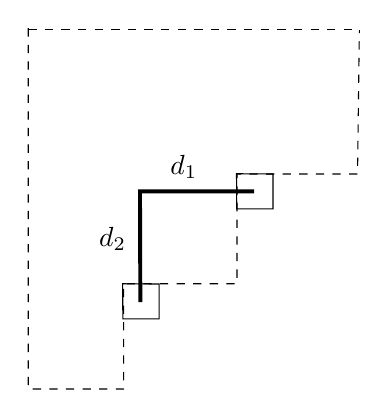
\begin{tikzpicture}[yscale=-1,scale=0.04,baseline={([yshift=-.5ex]current bounding box.center)}]
\begin{scope}[shift={(0.00mm,719.29mm)}]
% path id='path3338'
% path spec='m 162.85714,-399.06635 0,1145.71431 302.85715,0 0,-334.2857 360,0 0,-348.57146 382.85711,0 5.7143,-454.28572'
\draw [fill=none,draw=black,dashed] (162.86mm,-399.07mm)
-- ++(0.00mm,1145.71mm)
-- ++(302.86mm,0.00mm)
-- ++(0.00mm,-334.29mm)
-- ++(360.00mm,0.00mm)
-- ++(0.00mm,-348.57mm)
-- ++(382.86mm,0.00mm)
-- ++(5.71mm,-454.29mm)
;
% path id='path3340'
% path spec='m 162.85714,-396.2092 1051.42856,0 1e-4,6.33928'
\draw [fill=none,draw=black,dashed] (162.86mm,-396.21mm)
-- ++(1051.43mm,0.00mm)
-- ++(0.00mm,6.34mm)
;
% path id='path4161'
% path spec='M 824.28572,63.07651 940,63.79079 l 0,110.71429 -115,0 z'
\draw [fill=none,draw=black] (824.29mm,63.08mm)
-- (940.00mm,63.79mm)
-- ++(0.00mm,110.71mm)
-- ++(-115.00mm,0.00mm)
-- cycle
;
% path id='path4163'
% path spec='m 462.65115,412.44711 115.71428,0.71428 0,110.71429 -115,0 z'
\draw [fill=none,draw=black] (462.65mm,412.45mm)
-- ++(115.71mm,0.71mm)
-- ++(0.00mm,110.71mm)
-- ++(-115.00mm,0.00mm)
-- cycle
;
% path id='path4167'
% path spec='M 518.90014,412.43922 517.709,119.20535 825.48283,118.9091'
\draw [fill=none,draw=black, line width = 0.5mm] (518.90mm,470.44mm)
-- (517.71mm,119.21mm)
-- (880.48mm,118.91mm)
;
\node [black] at (657.10mm,40.28mm) { $d_1$ };
\node [black] at (430.53mm,270.26mm) { $d_2$ };
\end{scope}
\end{tikzpicture}
